\section{0x11\ 基础\ Misc}
\label{sec:0x11}

\subsection{常用常数表}

% 原 HTML：<img src="https://cdn.luogu.com.cn/upload/image_hosting/tmzjcvie.png" style="zoom:67%;" />
\begin{center}
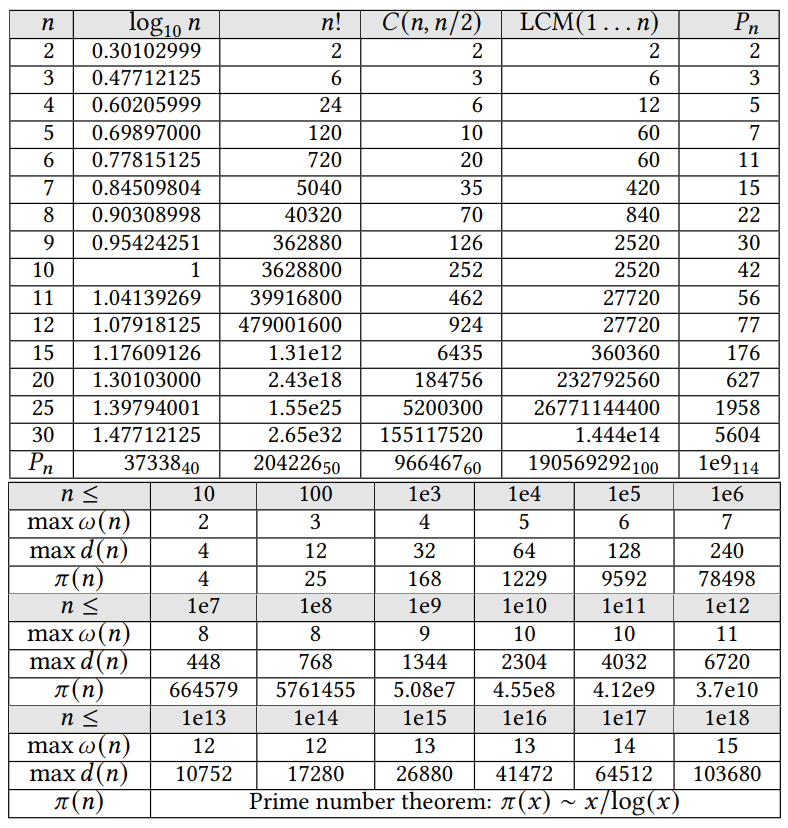
\includegraphics[width=0.8\textwidth]{contents/0x10 基础/figures/0x11 常数表.png}
\end{center}

\subsection{常用公式}

\subsubsection{日期公式}

\InputCode{cpp}{contents/0x10 基础/code/0x11 日期公式.cpp}

\subsubsection{xorshift}

\InputCode{cpp}{contents/0x10 基础/code/0x11 xorshift.cpp}

\subsubsection{xorsum}

\[
\operatorname{xor}_{i = 1}^n i = \begin{cases}
n, & n \bmod 4 = 0 \\
1, & n \bmod 4 = 1 \\
n + 1, & n \bmod 4 = 2 \\
0, & n \bmod 4 = 3
\end{cases}
\]

\InputCode{cpp}{contents/0x10 基础/code/0x11 xorsum.cpp}

\subsubsection{Sum of Powers}

\[
\begin{gathered}
\sum_{i = 1}^n i^2 = \frac{n(n + 1)(2n + 1)}{6}, \quad \sum_{i = 1}^n i^3 = \left( \frac{n(n + 1)}{2} \right)^2 \\
\sum_{i = 1}^n i^4 = \frac{n(n + 1)(2n + 1)(3n^2 + 3n - 1)}{30} \\
\sum_{i = 1}^n i^5 = \frac{n^2(n + 1)^2(2n^2 + 2n - 1)}{12}
\end{gathered}
\]

\subsection{常用配置}

\subsubsection{makefile}

\begin{minted}{make}
CXXFLAGS = -std=c++23 -O2 -Wall -fsanitize=undefined

# -D_GLIBCXX_DEBUG : STL debug mode
# -fsanitize=address : 内存错误检查
# -fsanitize=undefined : UB 检查
\end{minted}

\subsubsection{pragma}

\begin{minted}{cpp}
#pragma GCC optimize("O3,unroll-loops")
#pragma GCC target("avx2")
\end{minted}

\subsubsection{ulimit}

\begin{minted}{bash}
ulimit -s 1048576
\end{minted}

\subsubsection{Linux 对拍脚本}

需要 \texttt{chmod +x cmp.sh}，然后才能 \texttt{./cmp.sh}。

\begin{minted}{bash}
while true; do
    ./gen >0.in
    ./obj <0.in >1.out
    ./std <0.in >2.out
    let cnt=cnt+1; echo "Test $cnt:"
    if diff 1.out 2.out; then
        echo ac
    else
        echo wa
        break;
    fi
done
\end{minted}

\subsubsection{Windows 对拍程序}

\begin{minted}{cpp}
#include <bits/stdc++.h>
int main() {
    int T = 100;
    for (int i = 1; i <= T; i ++) {
        system("gen.exe >0.in");
        system("obj.exe <0.in >1.out");
        system("std.exe <0.in >2.out");
        std::cout << "Test " << i << ":\n";
        if (system("fc 1.out 2.out")) {
            std::cout << "wa\n";
            break;
        } else {
            std::cout << "ac\n";
        }
    }
}
\end{minted}

\subsection{随机数据生成}

\subsubsection{生成区间 [l,r] 中的随机整数}

\InputCode{cpp}{contents/0x10 基础/code/0x11 生成区间 [l,r] 中的随机整数.cpp}

\subsubsection{生成区间 [l,r) 中的随机浮点数}

\InputCode{cpp}{contents/0x10 基础/code/0x11 生成区间 [l,r) 中的随机浮点数.cpp}

\subsubsection{生成互不相同的随机整数}

\InputCode{cpp}{contents/0x10 基础/code/0x11 生成互不相同的随机整数.cpp}

\subsubsection{生成随机树}

\begin{itemize}
\item 均匀随机树的期望直径为 $\mathcal{O}(\sqrt{n})$ 级别。
\end{itemize}

\InputCode{cpp}{contents/0x10 基础/code/0x11 生成随机树.cpp}

\subsection{常用库函数重载}

\subsubsection{i128}

重载了 \texttt{\_\_int128} 的标准输入输出流。

\InputCode{cpp}{contents/0x10 基础/code/0x11 i128.cpp}

\subsubsection{整数除法精确取整}

\InputCode{cpp}{contents/0x10 基础/code/0x11 整数除法精确取整.cpp}

\subsubsection{取最值}

\InputCode{cpp}{contents/0x10 基础/code/0x11 取最值.cpp}

\subsubsection{取模}

\InputCode{cpp}{contents/0x10 基础/code/0x11 取模.cpp}

\subsubsection{精确开根号}

\InputCode{cpp}{contents/0x10 基础/code/0x11 精确开根号.cpp}

\subsubsection{精确取对数}

\InputCode{cpp}{contents/0x10 基础/code/0x11 精确取对数.cpp}

\subsubsection{快读}

\InputCode{cpp}{contents/0x10 基础/code/0x11 快读.cpp}

\subsubsection{超级快读}

\InputCode{cpp}{contents/0x10 基础/code/0x11 超级快读.cpp}

\subsection{高精度}

\InputCode{cpp}{contents/0x10 基础/code/0x11 高精度.cpp}

\subsection{分数类}

\InputCode{cpp}{contents/0x10 基础/code/0x11 分数类.cpp}

